%%%%%%%%%%%%%%%%%%%%%%%%%%%%%%%%%%%%%%%%%%%%%%%%%%%%%%%%%%%%%%%%%%%%%%
% How to use writeLaTeX: 
%
% You edit the source code here on the left, and the preview on the
% right shows you the result within a few seconds.
%
% Bookmark this page and share the URL with your co-authors. They can
% edit at the same time!
%
% You can upload figures, bibliographies, custom classes and
% styles using the files menu.
%
%%%%%%%%%%%%%%%%%%%%%%%%%%%%%%%%%%%%%%%%%%%%%%%%%%%%%%%%%%%%%%%%%%%%%%

\documentclass[12pt]{article}

\usepackage{sbc-template}

\usepackage{graphicx,url}
\usepackage{placeins}

\usepackage[brazil]{babel}   
\usepackage[utf8]{inputenc}  

\usepackage{hyperref}


%Inclui () nas citações
\usepackage[alf]{abntex2cite}




     
\sloppy

\title{Classificação de células tumorais em imagens\\ histopatológicas utilizando Deep Learning}

\author{Breno C. Zukowski\inst{1}, Lucas B. Figueira\inst{1}}


\address{Faculdade de Tecnologia de Ribeirão Preto - (FATEC)\\
  Ribeirão Preto, SP -- Brasil
  \email{breno.marques@fatec.sp.gov.br, lucas.figueira@fatec.sp.gov.br}}

\begin{document}

\maketitle

\begin{abstract}
  Diagnosing breast cancer can be challenging and laborious even for well-trained professionals.
  Inexperienced physicians and disagreement among histopathologists are primary causes of misdiagnosis
  that compromise patient care. With decision support computer systems using deep learning, it is possible to guarantee better results for this process. This article demonstrates the use
  of a deep learning model that uses YOLOv5 to validate the effectiveness of state-of-the-art computer vision methods for detecting malignant tumors in medical images.
\end{abstract}

\begin{resumo}
  O diagnóstico de câncer de mama pode ser desafiador e laborioso mesmo para profissionais bem treinados.
  Médicos inexperientes e discordância entre histopatologistas são causadores primários de diagnósticos errôneos
  que comprometem o tratamento de pacientes. Com sistemas computacionais de apoio a decisão utilizando deep learning, é possível garantir melhores resultados para este processo. Este artigo demonstra a utilização
  de um modelo de aprendizagem profunda que utiliza YOLOv5 para validar a eficácia de métodos de visão computacional de estado da arte para detecção tumores malignos em imagens médicas.
\end{resumo}


\section{Introdução}

O câncer de mama é a mais recorrente neoplasia maligna em mulheres ao redor do mundo. Apenas em 2020 foram realizados 2,3 milhões de diagnósticos e 685.000 mortes foram registradas \cite{who2021}. No Brasil, o cenário é similar: no mesmo ano a ordem de incidência estava prevista para cerca de 600.000 casos \cite{inca2018}. A análise de imagens histológicas está entre os mais utilizados métodos de diagnóstico da atualidade. Porém, existem deficiências associadas ao método provenientes do trabalho humano desenvolvido para realizá-lo. Falhas estas, que podem levar a diagnósticos errados e agravamento do quadro de saúde do paciente em decorrência da falta de tratamento imediato. Mesmo quando bem sucedidos, a análise humana demanda uma grande carga de esforço e tempo que poderiam ser mitigados com auxílio de visão computacional e deep learning.

Segundo \citeonline{tiezzi2020}, uma série de fatores podem ser descritos como métodos de predição de prognóstico, sendo atualmente utilizados no contexto clínico para determinação de tratamento, em especial para utilização de drogas antineoplásicas. Dentre eles destacam-se critérios clínicos, histológicos e utilização de marcadores tumorais. Abordando o critério histológico, temos o grau de diferenciação tumoral, baseado no sistema de escore de Nottingham (NGS), que, apesar de ser considerado um potente método de predição, recebe críticas em relação à sua baixa reprodutibilidade, provavelmente devido ao seu caráter subjetivo e processamento pré-analítico da amostra. Dessa forma, gera ampla discordância entre histologistas que o aplicam, o que impacta diretamente no prognóstico do paciente e na decisão clínica de administrar ou não a quimioterapia sistêmica \cite{tiezzi2020}.
Alternativas de métodos com biologia molecular vêm sendo propostas para inferir com maior acurácia o estágio de agressividade da doença de forma a evitar desvios de diagnóstico. Entretanto, essas são técnicas de alto custo, inviáveis em muitas situações, principalmente em países subdesenvolvidos.

Atualmente, as técnicas de aprendizado de máquina vêm ganhando espaço em diversas áreas e aplicações. Na medicina, já são importantes métodos de auxílio ao diagnóstico de imagens radiológicas \cite{hu2018}. Diversos modelos computacionais têm sido desenvolvidos nos últimos anos utilizando aprendizagem profunda para concretizar sistemas de apoio ao diagnóstico. Grupos de pesquisa ao redor do mundo têm desenvolvido soluções de aprendizado de máquina utilizando técnicas diversas de {\it Deep Learning}, que, apesar de rápidas e geralmente acuradas, apenas oferecem mapas de calor e pontos de atenção, informações insuficientes para interpretação concreta e justificativa do diagnóstico oferecido pela máquina, o que não é adequado para sistemas de apoio à decisão médica \cite{li2021}.

Vê-se, portanto, nas CNNs (do inglês, Convolutional Neural Network) de classificação de objetos em imagens, uma solução viável para análise de recortes específicos de tecido com a quantidade de informação e assertividade adequadas para auxílio ao diagnóstico médico. Pois a partir delas é possível segmentar e classificar regiões de interesse com as informações necessárias para evidenciar a presença de tumores malignos com eficiência.

O presente artigo propõe um modelo  de aprendizagem profunda para a segmentação de áreas de interesse e posterior classificação de imagens histológicas visando apoiar o diagnóstico de câncer de mama.


\section{Revisão bibliográfica}

\subsection{Introdução}
Para justificar sua utilização é primeiro importante entender os conceitos que embasam as CNN's, técnicas estas utilizadas como base para  a realização da detecção e classificação de objetos. Portanto entendemos como CNN: algoritmos de aprendizagem profunda especializados em processamento e classificação de imagens. Segundo \cite{Goodfellow-et-al-2016} redes neurais convolucionais são um tipo especializado de rede neural para processamento de dados organizados topologicamente em grades, que através de operações matemáticas chamadas convoluções, são capazes de extrair características principais das entradas utilizando filtros (kernels), garantindo eficiência e redução de custos computacionais para a classificação.

Diferentemente de outros tipos de dados, imagens possuem a propriedade de {\it invariância de tradução} \cite{Aggarwal18}, ou seja, transmitem a mesma informação sobre o objeto independentemente das variações do contexto. No entanto, existem características espaciais, de luz, sombra, perspectiva, cenário, entre outras variáveis, que alteram significantemente a matriz de pixels que constituem a imagem do objeto de estudo. Enquanto para um ser humano distinguir um objeto qualquer no espaço independente da posição, incidência de luz ou cenário em que este se encontra seja uma tarefa trivial, para um computador esta tem um custo elevado de execução. Sendo assim, é necessário que se utilize de técnicas que permitam a extração de características mais objetivas e com dados relevantes para a análise, evitando imprecisões que não contribuem para a classificação do objeto desejado.

Em geral, uma CNN apenas difere de uma rede neural densa totalmente conectada por apresentar camadas destinadas ao processamento das imagens que serão analisadas. Apresentando camadas de convolução, ativação, pooling, tal como apresentado na Figura \ref{fig:cnn} para finalmente enviar esses dados para uma rede neural densa que fará a classificação.


% Revisar caption da figura
\begin{figure}[ht]
  \centering
  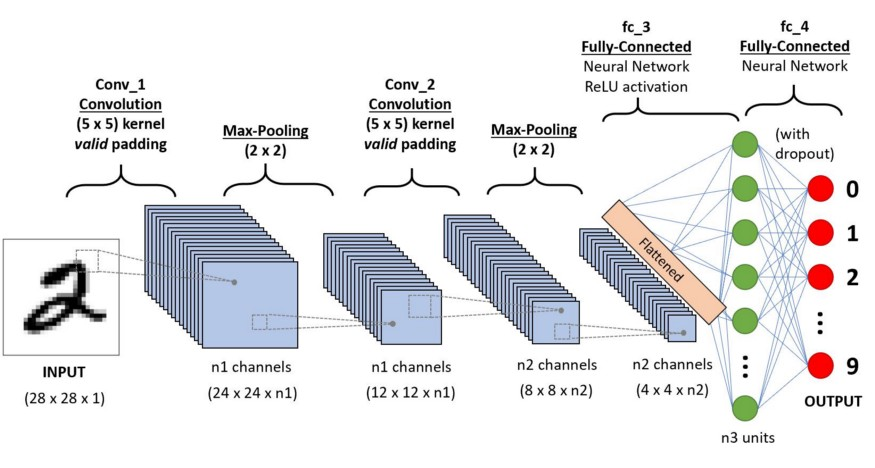
\includegraphics[width=1\textwidth]{images/CNN.jpeg}
  \caption{O fluxo básico de uma CNN e suas diversas camadas. Fonte: Introduction to Convolutional Neural Networks (CNN). Disponível em: https://www.analyticsvidhya.com/blog/2021/05/convolutional-neural-networks-cnn/}
  \label{fig:cnn}
\end{figure}



\subsection{Convolução}

Em aplicações de aprendizagem de máquina a convolução é comumente interpretada como uma operação entre a imagem $I$ e o kernel $K$, matrizes multidimensionais que ao serem convolucionadas resultarão em uma nova matriz que chamamos de {\it{feature map}} ou mapa de características. Quando tomamos por exemplo uma convolução de matrizes bidimensionais temos de levar em consideração certas propriedades matemáticas que não se traduzem bem para cenários práticos de aprendizagem profunda. Dessa forma, muitos {\it frameworks} de redes neurais implementam uma função similar chamada
correlação cruzada ({\it cross-correlation}), que é em suma a mesma operação sem a rotação do kernel. Sendo definida pela seguinte função:

$$ S(i,j) = (I * K) (i,j) = \sum_m \sum_n I(i + m, j + n) K(m, n)  $$


Em termos gerais, basta que multiplique-se os valores das posições equivalentes do kernel nas coordenadas da imagem analisada, posteriormente soma-se todos os resultados para que se obtenha um valor único na posição definida $(i,j)$ do {\it feature map}. É possível visualizar este processo com clareza na Figura \ref{fig:convolution}.

O kernel é constituído por parâmetros que filtram certas características desejadas do {\it input}, uma rede neural convolucional pode apresentar diversas camadas de convolução para extração de características diferentes. As primeiras camadas em geral extraem características mais gerais, como bordas e contornos, enquanto as camadas posteriores extraem características mais específicas e abstratas.


\begin{figure}[ht]
  \centering
  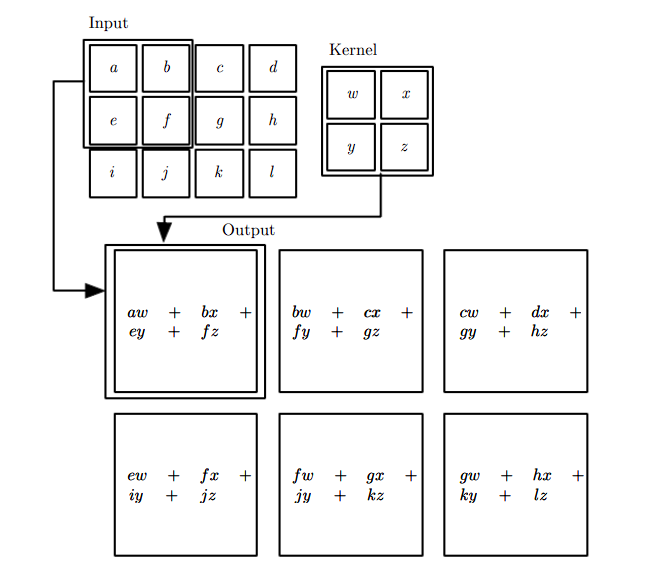
\includegraphics[width=0.8\textwidth]{images/convolution.png}
  \caption{O processo de convolução sem rotação explicado graficamente. Imagem retirada do livro {\it Deep Learning} \cite{Goodfellow-et-al-2016}. Onde é possível perceber que o output é restringido apenas as posições compreendidas dentro da imagem por todos os parâmetros do kernel. São desenhadas caixas para indicar as saídas referentes a multiplicação e somatório das posições equivalentes do kernel à imagem.}
  \label{fig:convolution}
\end{figure}


\subsection{Pooling}

Apesar da efetividade de destaque de características provenientes da técnica de convolução, o {\it feature map} ainda destaca demasiadamente informações sobre localização espacial das {\it features} na saída, gerando uma variável extra a ser analisada (característica e posição) que prejudica a invariância de tradução da imagem. É mais relevante em geral para o modelo, compreender que a característica desejada está presente no objeto, do que sua posição especificamente \cite{Goodfellow-et-al-2016}. Portanto, em um fluxo comum de CNN é necessário que após o processo de convolução e aplicação da função de ativação (transformação não linear realizada ao longo do sinal de entrada), seja realizada uma operação que permita suavizar a saída classificada. A esta técnica damos o nome de {\it pooling}.

A camada de {\it pooling} substitui a saída do {\it feature map} por uma estatística aproximada das informações desejadas para a rede neural densa, garantindo uma aproximação de invariância que permite melhores resultados para as operações realizadas nesse conjunto de dados \cite{Goodfellow-et-al-2016}.

Existem diversas funções de {\it pooling}, as duas mais comuns são: {\it Average Pooling} e {\it Max Pooling}. Seus respectivos algoritmos tem propósitos distintos, entretanto ambos cumprem o papel de filtrar o {\it feature map} de tal forma a reduzir a dimensionalidade da imagem e destacar características principais a serem processadas pela rede neural densa. Gerando um novo mapa de características que chamamos de {\it pooled feature map}.

\subsection{Detecção unificada de objetos em tempo real com YOLO}

Segundo \citeonline{Redmon2015} alternativas conhecidas de classificadores como R-CNN's ({\it Regions with Convolutional Neural Networks}) utilizam métodos para primeiro gerar potenciais caixas delimitadoras ({\it do inglês, bounding boxes}) em uma imagem e posteriormente rodar um classificador para as áreas segmentadas. Após as classificações, é aplicado ainda pós-processamento para refinar as delimitações, eliminar duplicações e possíveis imprecisões. Esse tipo de modelo, devido a sua complexidade, torna-se lento e de difícil otimização pois cada componente individual de sua composição deve ser treinado separadamente.

Com a proposta de ser um classificador de objetos de alta performance, YOLO propõe uma abordagem diferente das convencionais entregando velocidade e acurácia com custo computacional reduzido, além de uma arquitetura escalável devido a sua simplicidade. O modelo YOLO reformula o problema de detecção de objetos para um problema de regressão, utilizando apenas uma rede neural para criar {\it bounding boxes} e indicar as probabilidades dos objetos estarem presentes nessas imagens \cite{Redmon2015}.

Para tal, o sistema divide a imagem de entrada em um grid $S x S$. Caso o centro da imagem caia em uma determinada célula, esta fica responsável por fazer a detecção daquele objeto, por sua vez esta prevê $B$ caixas delimitadoras e valores de confiança para cada uma delas formalmente definidos por $Pr(Object) * IOU^{truth}_{pred}$. Se não existir objetos na respectiva célula o fator de confiança é determinado como zero, do contrário a confiança de predição é representada pelo IOU ({\it Intersection Over Union}) da {\it bounding box} predita em relação a qualquer caixa delimitadora tomada como verdade absoluta \cite{Redmon2015}.

Ademais, cada {\it bounding box} é composta por 5 valores: $x, y, w, h$ e confiança \cite{Redmon2015}. Onde $x, y$ são as coordenadas do centro da caixa delimitadora, $w, h$ são a largura e altura relativas a imagem completa. Vale ressaltar que são preditas também $C$ potenciais classes condicionais por célula e sua probabilidade é dada por $Pr(Class_i | Object)$ e apenas se prevê um único conjunto probabilidades de classe por célula do grid, independente de quantas {\it bounding boxes} foram demarcadas no processo \cite{Redmon2015}.

Durante o momento de testes são multiplicados as classes condicionais e as confianças individuais de cada caixa predita como visto em (\ref{testing_expression}) o que dá os fatores de confiança específicos de cada {\it bounding box} e por sua vez o fluxo pode ser compreendido na totalidade a partir da Figura \ref{fig:yolo}.

\begin{equation}
  \label{testing_expression}
  Pr(Class_i|Object) * Pr(Object) * IOU^{truth}_{pred} = Pr(Class_i) * IOU^{truth}_{pred}
\end{equation}

\begin{figure}[ht]
  \centering
  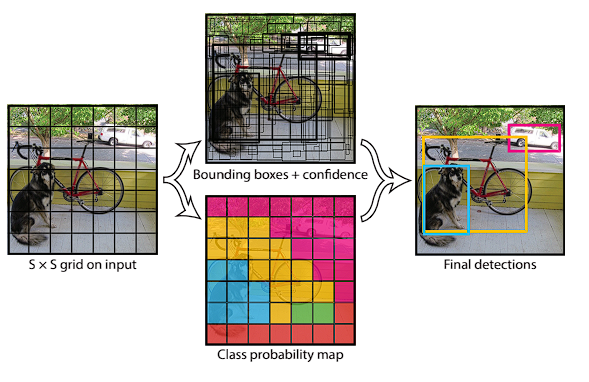
\includegraphics[width=0.7\textwidth]{images/yolo.png}
  \caption{Imagem retirada do artigo de \citeonline{Redmon2015}. Onde é possível ver com clareza o processo de separação da imagem em pequenas células em um grid $S x S$, a plotagem de $B$  bounding boxes, o mapa de $C$ probabilidades de classe e por fim um exemplo de detecção final.}
  \label{fig:yolo}
\end{figure}

\FloatBarrier

\section{Materiais e Métodos}

Para concepção do modelo de detecção, utilizou-se uma seleção de imagens oferecidas por um especialista da área derivadas do banco de imagens TCGA \footnote{Disponível em: \url{https://portal.gdc.cancer.gov/projects/TCGA-BRCA} Acessado em: 19/08/2022 }, {\it dataset} este que possui informações clínicas e histopatológicas de 1098 pacientes com câncer de mama e suas respectivas imagens histológicas \cite{tiezzi2020}.

Posteriormente, como é requisitado pela documentação oficial do YOLOv5 \cite{glenn_jocher_2022} em sua arquitetura, foram anotados os tumores presentes em cada imagem que participaria do sub-conjunto de treino com as ferramentas {\it LabelImg} \cite{tzutalin2015labelimg} e {\it Label Studio} \cite{labelStudio} que são capazes de gerar anotações de classes em formato adequado para o treinamento, que serão utilizadas como padrões de referência de verdade absoluta para o modelo.

Para o processo de treinamento foram utilizadas 57 imagens que totalizam 1224 de objetos da classe tumor anotados. Este se deu em 250 épocas com lotes de 16 imagens, valores estes arbitrários com embasamento em exemplos da literatura. Devido ao tamanho reduzido do {\it dataset} para o treinamento, foi-se utilizado o modelo pré-treinado YOLOv5s \cite{glenn_jocher_2022} como é recomendado pela própria documentação oficial da arquitetura. Ao completar-se o processo, é gerado o novo modelo com pesos atualizados que pode ser utilizado para a detecção de tumores malignos.

Ademais, realizou-se a execução do script de validação em lotes de 64 imagens no subconjunto destinado a essa finalidade, para se obter as métricas que compõem a performance do sistema. Por fim, foram executados alguns testes para verificar a eficácia de anotação do modelo de forma visual em imagens selecionadas arbitariamente. Todo o fluxo pode ser observado na Figura \ref{fig:methods}.

\begin{figure}[ht]
  \centering
  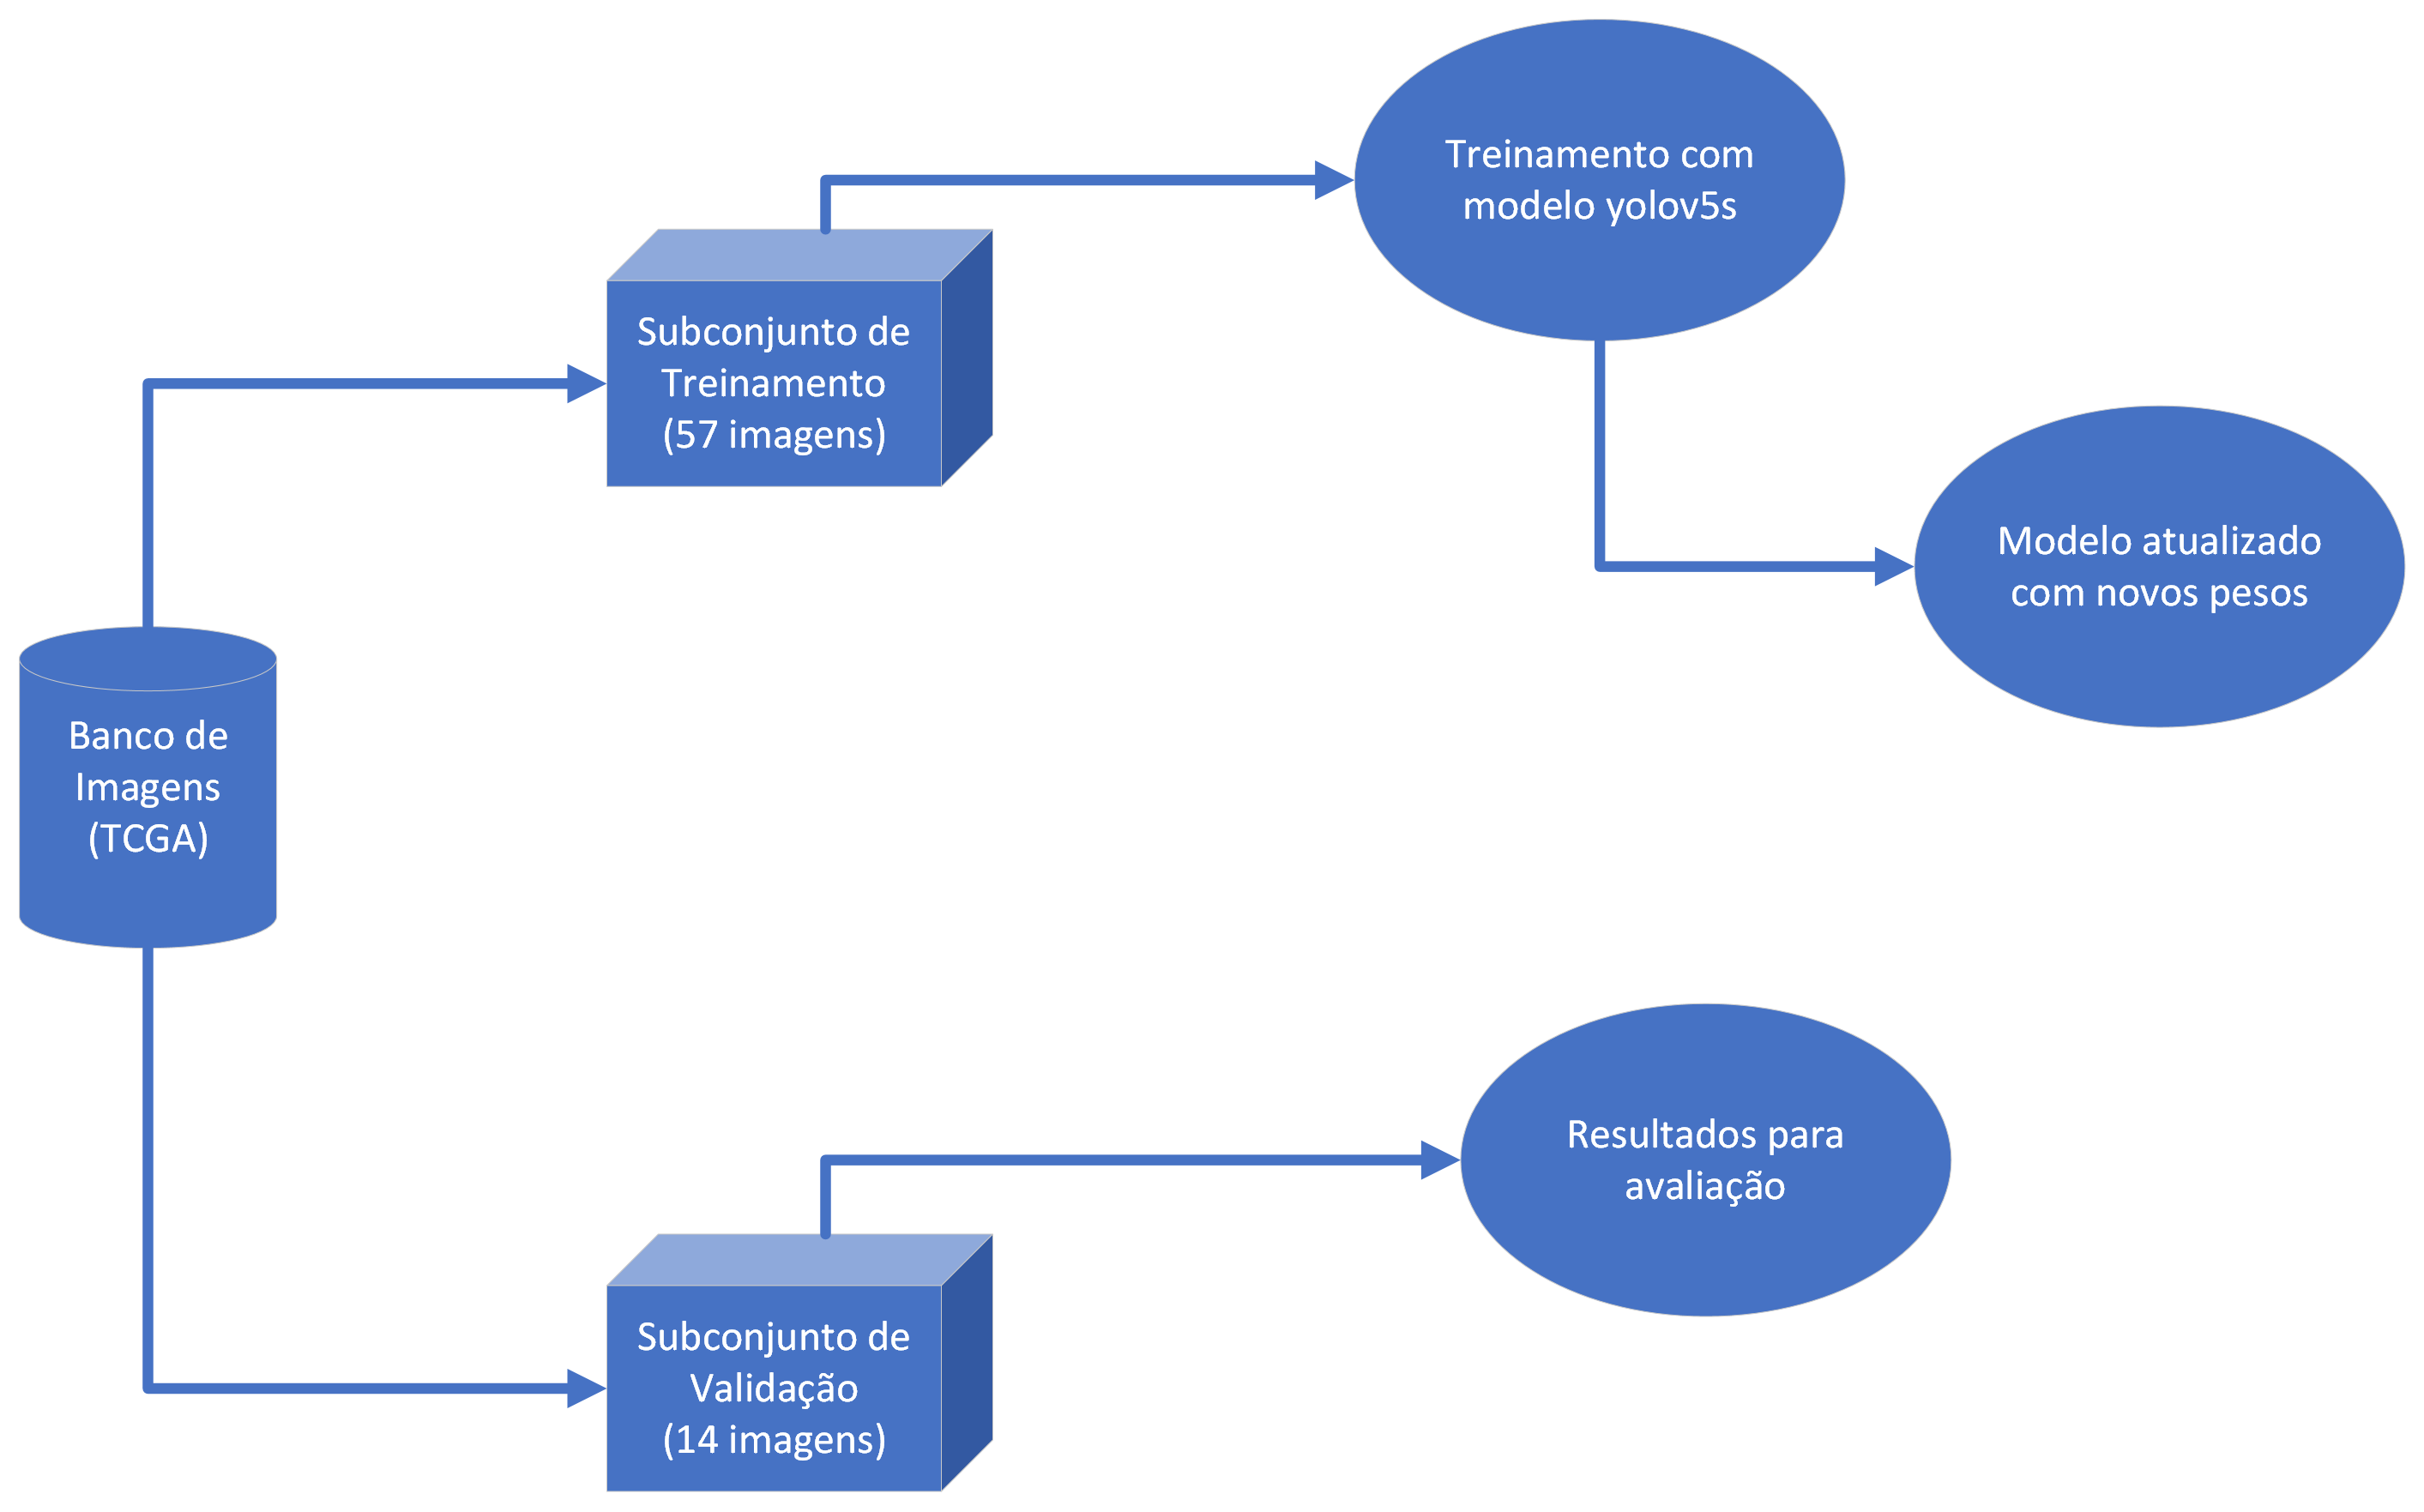
\includegraphics[width=0.9\textwidth]{images/methods.png}
  \caption{Fluxo do processo de treinamento e validação do modelo.}
  \label{fig:methods}
\end{figure}

\section{Resultados}

Após a avaliação de resultados gerados conseguimos obter a partir da matriz de confusão a acurácia de $81\%$. Como indicado na Figura \ref{fig:graph}. A precisão alcança o pico de 1.00 Ao se observar o balanço entre os gráficos de {\it precision} e {\it recall} entende-se as detecções relevantes estão até o nível de confiança de $0.7$, a partir daí o {\it recall} decai de forma expressiva indicando que o modelo já não mais apresenta assertividade em suas detecções.




\begin{figure}[ht]
  \centering
  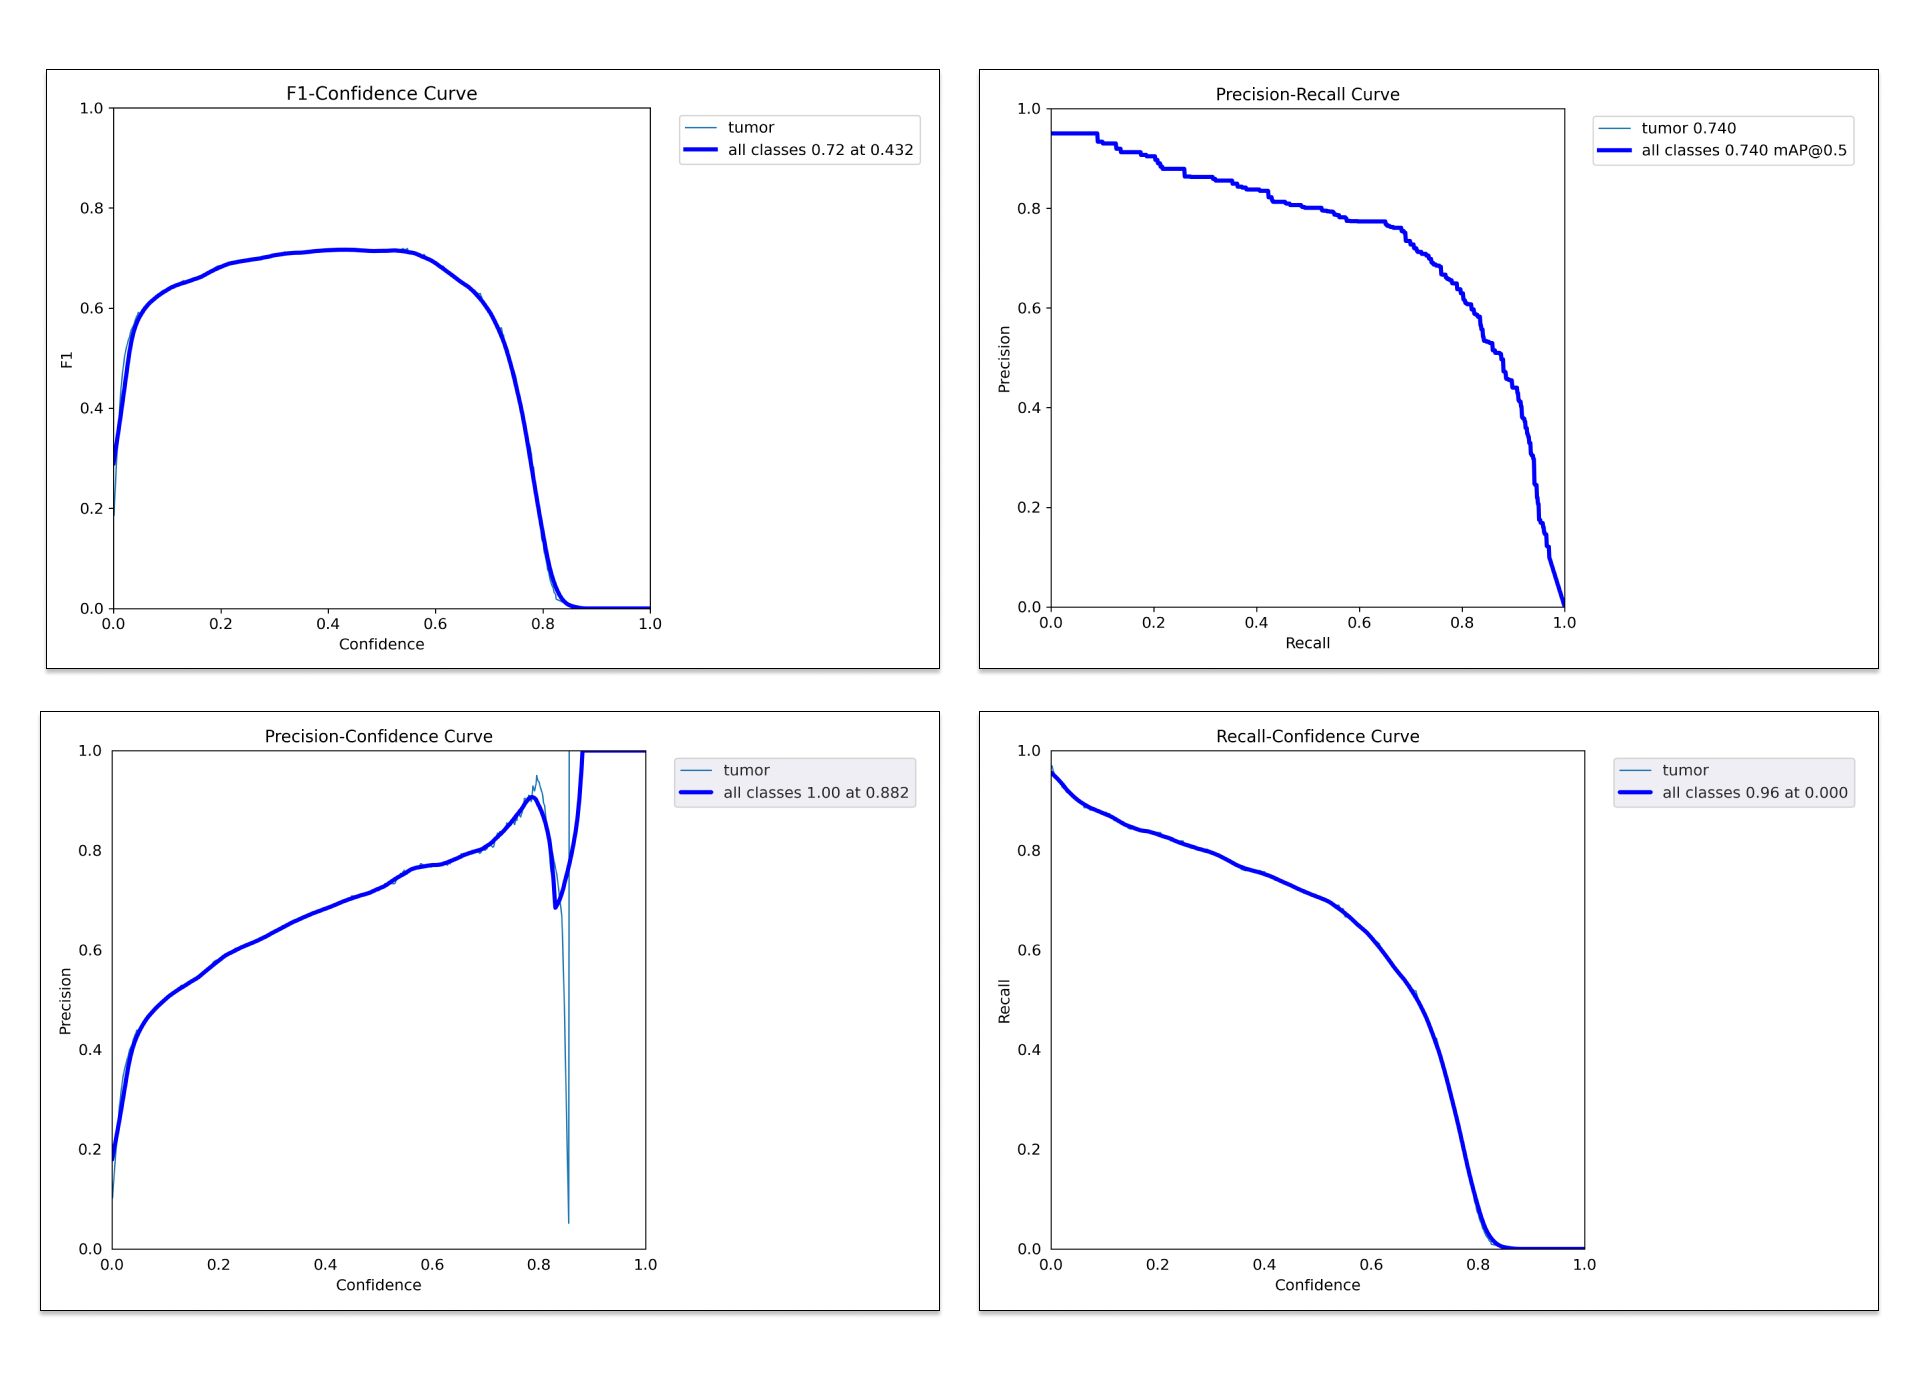
\includegraphics[width=1\textwidth]{images/graph_results.png}
  \caption{Gráficos de performances do modelo contendo respectivamente os gráficos relativos F1-Confiança, Precision-Recall, Precision-Confiança e Recall-Confiança.}
  \label{fig:graph}
\end{figure}

\FloatBarrier

\section{Conclusão}

\bibliographystyle{abnt}
\bibliography{sbc-template}

\end{document}